% !TEX program = xelatex

\documentclass{resume}
\usepackage{graphicx}
\usepackage{tabu}
\usepackage{multirow}
\usepackage{zh_CN-Adobefonts_external} % 
%\usepackage{zh_CN-Adobefonts_external} % Simplified Chinese Support using external fonts (./fonts/zh_CN-Adobe/)
%\usepackage{zh_CN-Adobefonts_internal} % Simplified Chinese Support using system fonts

\begin{document}
\pagenumbering{gobble} % suppress displaying page number

\Large{
  \begin{tabu}{ c l r }
   \multirow{5}{1in}{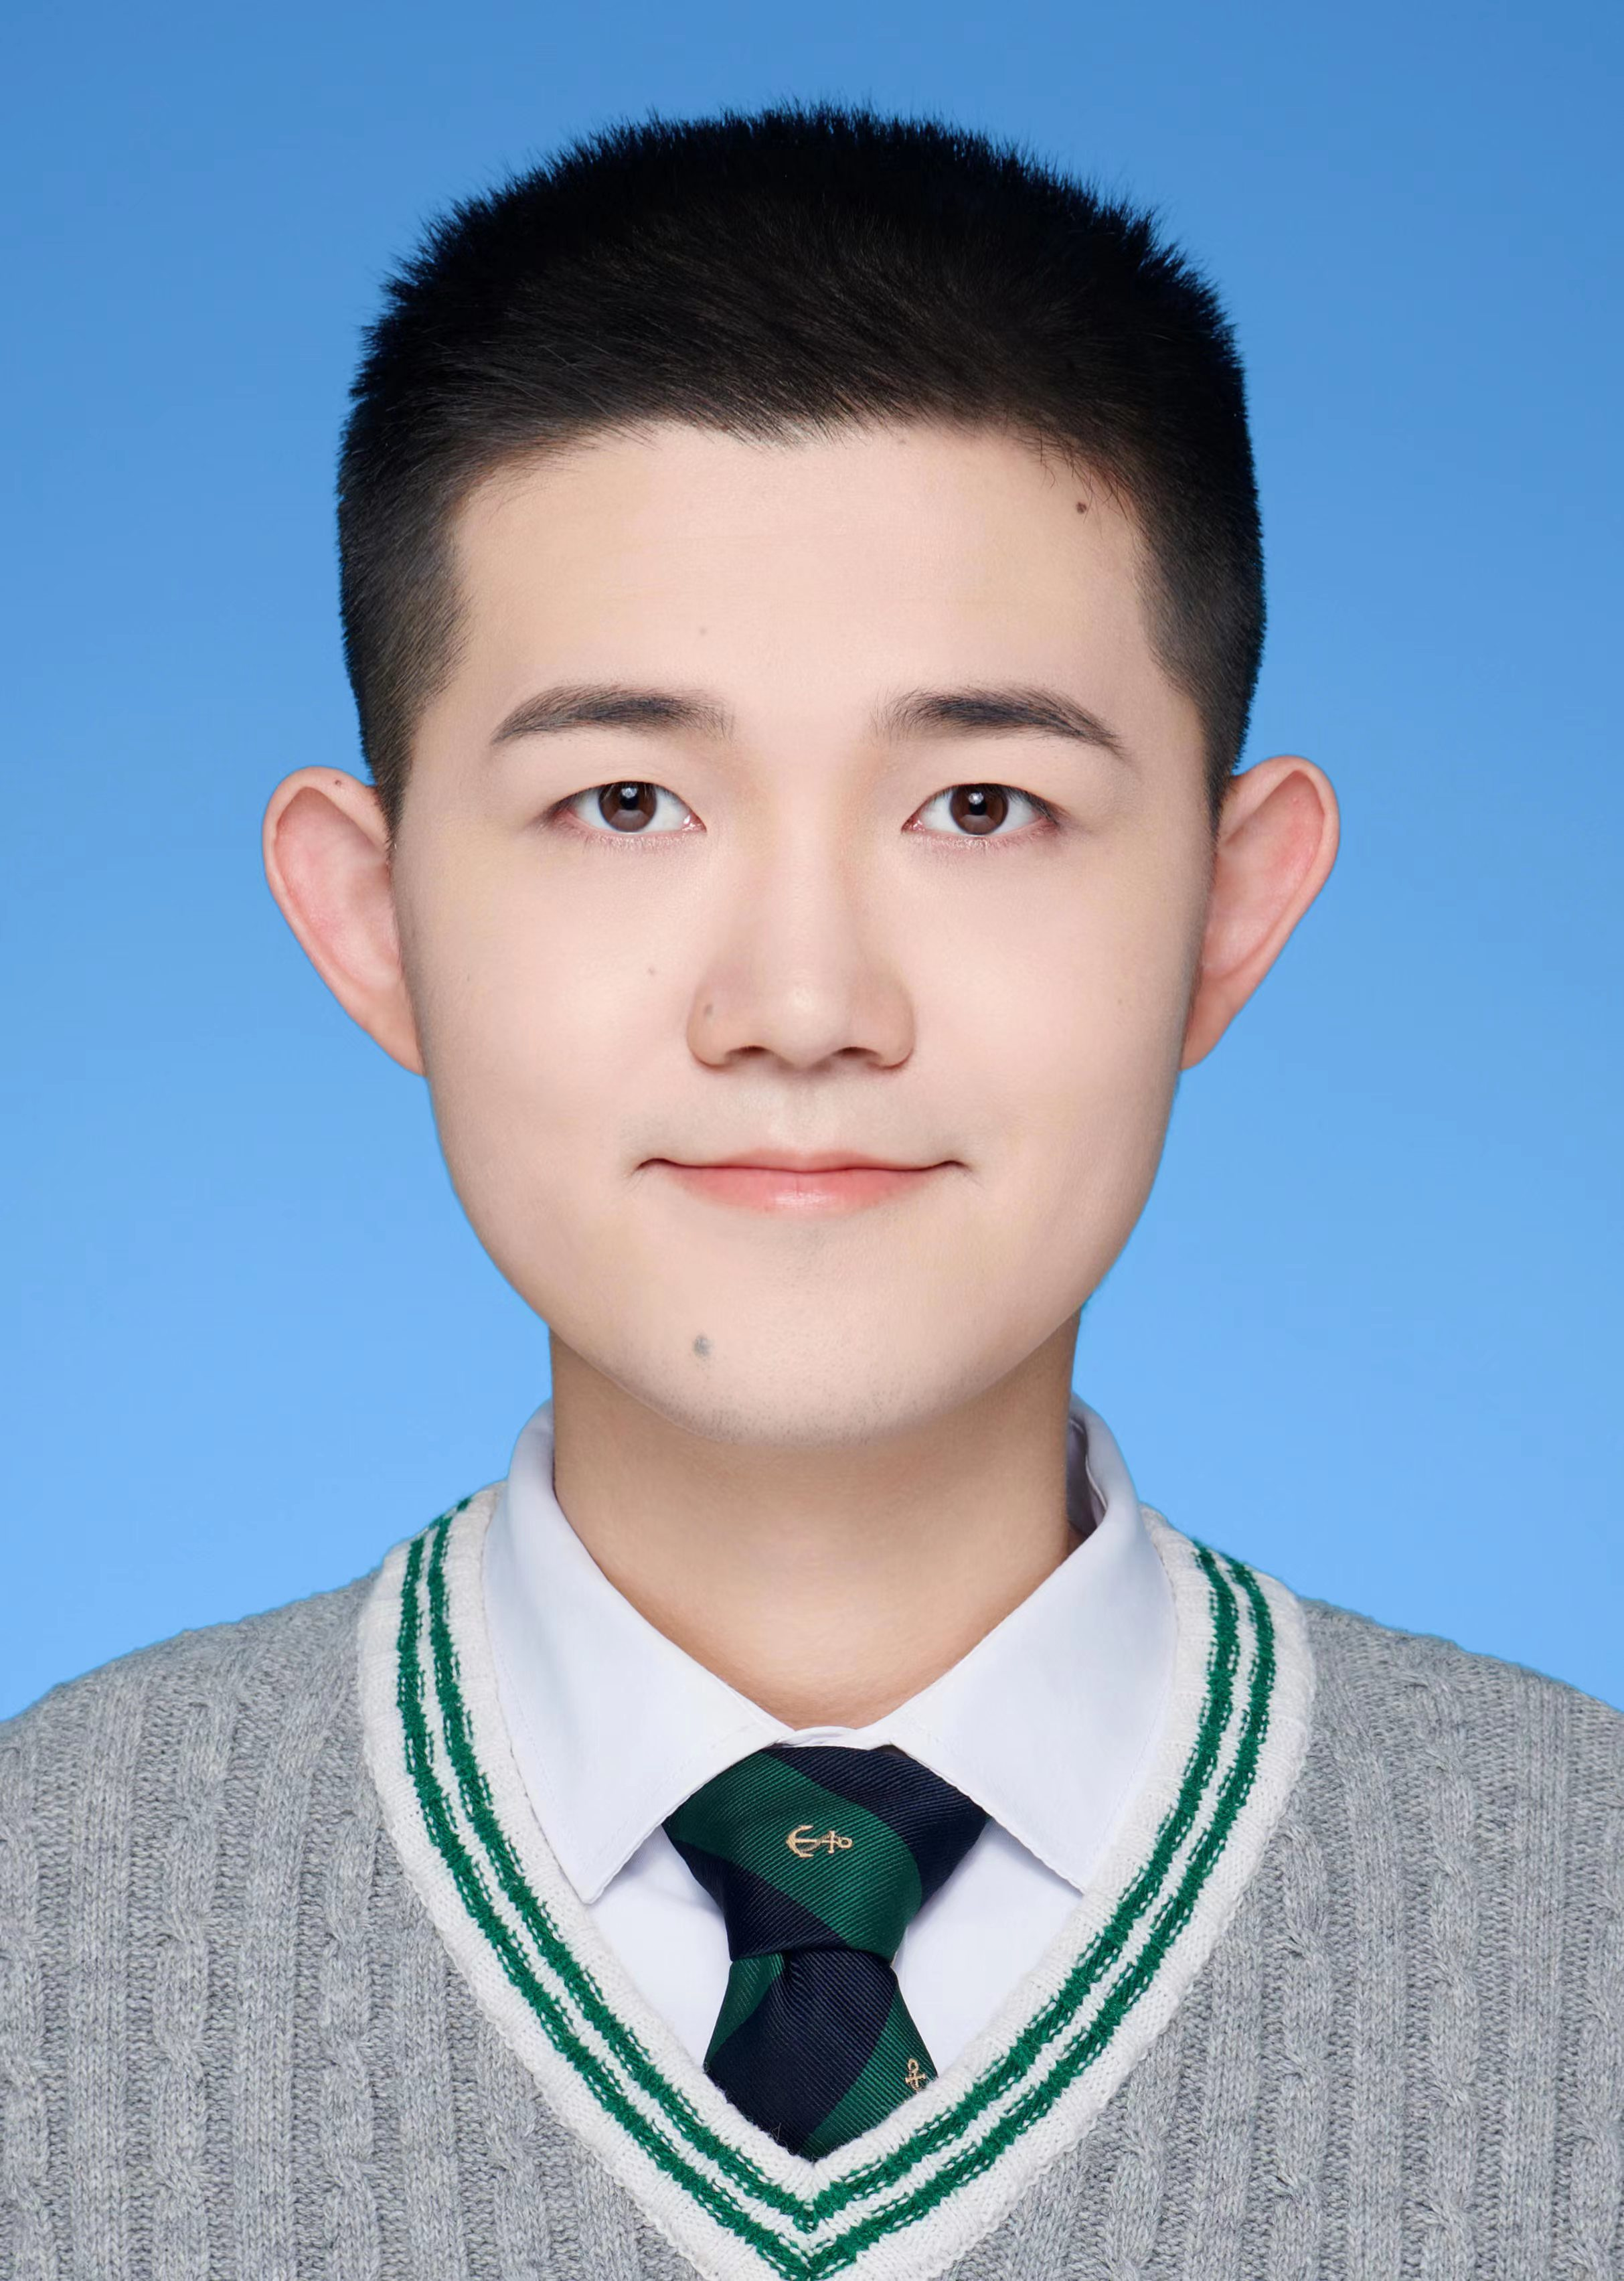
\includegraphics[width=0.88in]{avatar-college}} & \scshape{Ruan Yanhan} & \pbar{React}{0.8} \\
    & \email{ruanyanhan@whu.edu.cn} & \pbar{ES6}{0.8} \\
    & \phone{(+86) 173-1836-1969} & \pbar{WebGIS}{0.5} \\
    & \linkedin[yo yo]{https://www.linkedin.com/in/yo-yo-974516289/} & \pbar{Express}{0.6} \\
    & \github[gitee.com/yohoyh]{https://gitee.com/yohoyh} & \pbar{Jquery}{0.6}
  \end{tabu}
}

\section{\faGraduationCap\ Education}
\datedsubsection{\textbf{Wuhan University (WHU)}, Wuhan, China}{2022 -- Present}
\textit{Master student} in Civil and Hydraulic engineering , expected July 2024
\datedsubsection{\textbf{NORTHWEST A\&F UNIVERSITY (NWAFU)}, Shaanxi, China}{2018 -- 2022}
\textit{B.S.} in Water Resources and Hydropower Engineering

\section{\faUsers\ projects \& Experience}
% 横沙项目
\datedsubsection{\textbf{Carbon Neutralization Big Data Platform} Shanghai, China}{May. 2023 -- Present}
\role{work with government departments.}{React | Antd | Express | ECharts | Resium}
% Brief introduction: The platform aims to enable carbon-neutral assessment and agricultural land information management on the islands.The main technical highlights are as follows:
\begin{itemize}
  \item Utilizing modern ES6+ syntax: Enhancing development efficiency and code readability by leveraging the latest JavaScript syntax.
  \item Encapsulation of reusable utility functions: Throttling cesium re-render event, Debouncing clicks, axios interceptors, etc, improving code maintainability.
  \item Robust screen adaptation using relative units: By employing relative units, the project ensures strong screen adaptability for various devices and screen sizes.
  \item Login validation through Higher Order Components (HOC): easily apply this functionality to components that require login validation.
  \item Enhanced performance and user experience with lazy loading, optimize entity loading within a specified height range using hooks and throttling.
\end{itemize}

% 清美+宁夏
\datedsubsection{\textbf{Digital Rice Platform} Wuhan, China}{March. 2022 -- November. 2022}
\role{based on national key project}{Jquery | Express | ECharts | OpenLayers}
% Brief introduction: The platform aims to enable carbon-neutral assessment and agricultural land information management on the islands.The main technical highlights are as follows:
\begin{itemize}
  \item Regional intelligent management, detailed development document writing, effective management and development.
  \item The system conducts strict security verification and has good security precautions.
  \item Utilize dual-pointer algorithm to reduce time complexity from \(\mathbf{\mathit{o(n^{2})}}\) to \(\mathbf{\mathit{o(n)}}\), and preprocess remote sensing images for 150\% speed increase.
\end{itemize}

% Reference Test
%\datedsubsection{\textbf{Paper Title\cite{zaharia2012resilient}}}{May. 2015}
%An xxx optimized for xxx\cite{verma2015large}
%\begin{itemize}
%  \item main contribution
%\end{itemize}

% \section{\faCogs\ Skills}
% \begin{itemize}[parsep=0.5ex]
%   \item Programming Languages: C == Python > C++ > Java
%   \item Platform: Linux
%   \item Development: Web, xxx
% \end{itemize}

% \section{\faHeartO\ Honors and Awards}
% \datedline{\textit{\nth{1} Prize}, Award on xxx }{Jun. 2013}
% \datedline{Other awards}{2015}

\section{\faCalendarCheckO\ Awards}
\begin{itemize}[parsep=0.5ex]
  \item 2022 ZJU PAT - Professional Ability Test (95 / 100 score) 
  \item 2022 ACM-ICPC excellence-award \ \ \ \ \ \ \ \ \ \ \ \ \ \ \ \ \ \ \ \  • 2020 CMC second-prize
  \item 2020 MCM S-Award \ \ \ \ \ \ \ \ \ \ \ \ \ \ \ \ \ \ \ \ \ \ \ \ \ \ \ \ \ \ \ \ \ \ \ \ \ \ \ \ \ \ \ • 2021 2 software works
  % \item 
  % \item 
\end{itemize}

\section{\faPlusCircle\ Miscellaneous}
\begin{itemize}[parsep=0.5ex]
  \item CET-6: 539 score, daily conversations, skilled in reading English documents.
\end{itemize}

%% Reference
%\newpage
%\bibliographystyle{IEEETran}
%\bibliography{mycite}
\end{document}
